\documentclass{article}
\usepackage[utf8]{inputenc}
\usepackage{amsmath}
\usepackage{amsfonts}
\usepackage{graphicx}
\usepackage{todonotes}
\newcommand{\acc}{\text{acc}}
\newcommand{\conf}{\text{conf}}
\newcommand{\D}{\mathcal{D}}
\usepackage{hyperref}
\hypersetup{
    colorlinks=true,
    linkcolor=blue,
    filecolor=magenta,      
    urlcolor=blue,
    pdftitle={Overleaf Example},
    pdfpagemode=FullScreen,
}

\title{Distribution Shift Robustness}

\begin{document}

\maketitle

\section{Introduction}
%\todo{Train test mismatch => it's a way to simulate black swan examples. If you're robust to distribution shift, you're robust to black swan events.}
To illustrate distribution shift robustness, we revisit the previous chapter's scenario of a cats-vs-dogs classifier. This time, having trained and deployed your classifier on an app, let's say that you only use the app on genuine cats or dogs. When testing your app, you notice that somehow, the real-world accuracy is 20\%-30\% lower than the training dataset—perhaps your model is overfitting? You retrain your model, leaving aside some data for validation. Yet somehow the real-world accuracy is still 20\%-30\% lower than validation accuracy. This issue, you realize, isn't overfitting. Instead, it's likely that the model is performing poorly because of a distribution shift between training and real-world environments.

A distribution shift, or dataset shift, is when the training set and the testing set are sampled from a different underlying distribution. In other words, if there are systematic differences between the samples drawn from the training and testing distribution. Here, `testing' often refers to data seen in the real-world scenario, after the model has been deployed in an application. Distribution shifts are one of the largest problems in preventing widespread adoption of deep learning systems. For instance, in medicine, practitioners will first train a model on a large public dataset and then deploy it to a local hospital. However, there are many differences between the dataset and the local hospital. Some are deep, like underlying differences in population demographics. Others are simple, like a difference in brand of imaging equipment, leading to images of different aspect ratio or resolution. 

% Insert DSR here!
Similarly, self-driving cars may need to deal with unexpected weather conditions, like hail or fog, and social media algorithms need to keep pace with all the new slang being developed. For all of these reasons, it is crucial to ensure that our models perform well, even when the distribution shifts.

\section{Problem}
More formally, a distribution shift is when the training distribution does not match the testing distribution: $P_\text{train}(X,Y) \neq P_\text{test}(X,Y)$. Moreover, we can further subdivide distribution shifts into a few, non-exhaustive categories \cite{quinonero2009dataset}. In practice, some papers adhere to the specific terminology whereas other papers simply discuss ``distribution shift.''

\textbf{Label Shift}, also known as prior probability shift, is when $P_\text{train}(X|Y) = P_\text{test}(X|Y)$, but $P_\text{train}(Y) \neq P_\text{test}(Y)$. In other words, everything remains constant except for the label distributions $P_\text{train}(Y)$ and $P_\text{test}(Y)$. 

\textbf{Covariate Shift} is when $P_\text{train}(Y|X) = P_\text{test}(Y|X)$, but $P_\text{train}(X) \neq P_\text{test}(X)$. In other words, everything remains constant except for the input distributions $P_\text{test}(X)$ and $P_\text{train}(X)$. Most papers in deep learning which are described as solving ``distribution shift'' are actually solving covariate shift. This includes these notes, which will henceforth focus on covariate shift as well.

%\todo{@Chris, would be nice to have an `examples' or `in the wild' section here. Why is this a problem that's important, with concrete examples}

%\todo{@Chris, Would be nice to contextualize this in comparison to other safety issues. E.g. how does this differ from adversarial examples or data poisoning? (One answer: 'covariate shift' can't depend on the model, while adversarial examples generally do depend on the model)}

\subsection{Benchmarks}
Robustness to distribution shift is usually measured by performance on robustness benchmarks. Importantly, these benchmarks should only be used for testing models, not training models. We avoid training models on these benchmarks to ensure that the distribution shifts are somewhat representative of unforeseen distribution shifts. With the exception of WILDS, we focus robustness benchmarks designed to test the robustness of ImageNet classifiers.

\subsubsection{ImageNet-C}
\href{https://paperswithcode.com/sota/domain-generalization-on-imagenet-c}{ImageNet-C} \cite{hendrycks2019benchmarking}, which stands for “ImageNet Corruptions” is a benchmark created by modifying ImageNet. ImageNet-C applies fifteen common corruptions to ImageNet at five levels of severity each (for a total of 75 corruptions). The fifteen corruptions can be seen in figure \ref{fig:corruptions}.

\begin{figure}
    \centering
    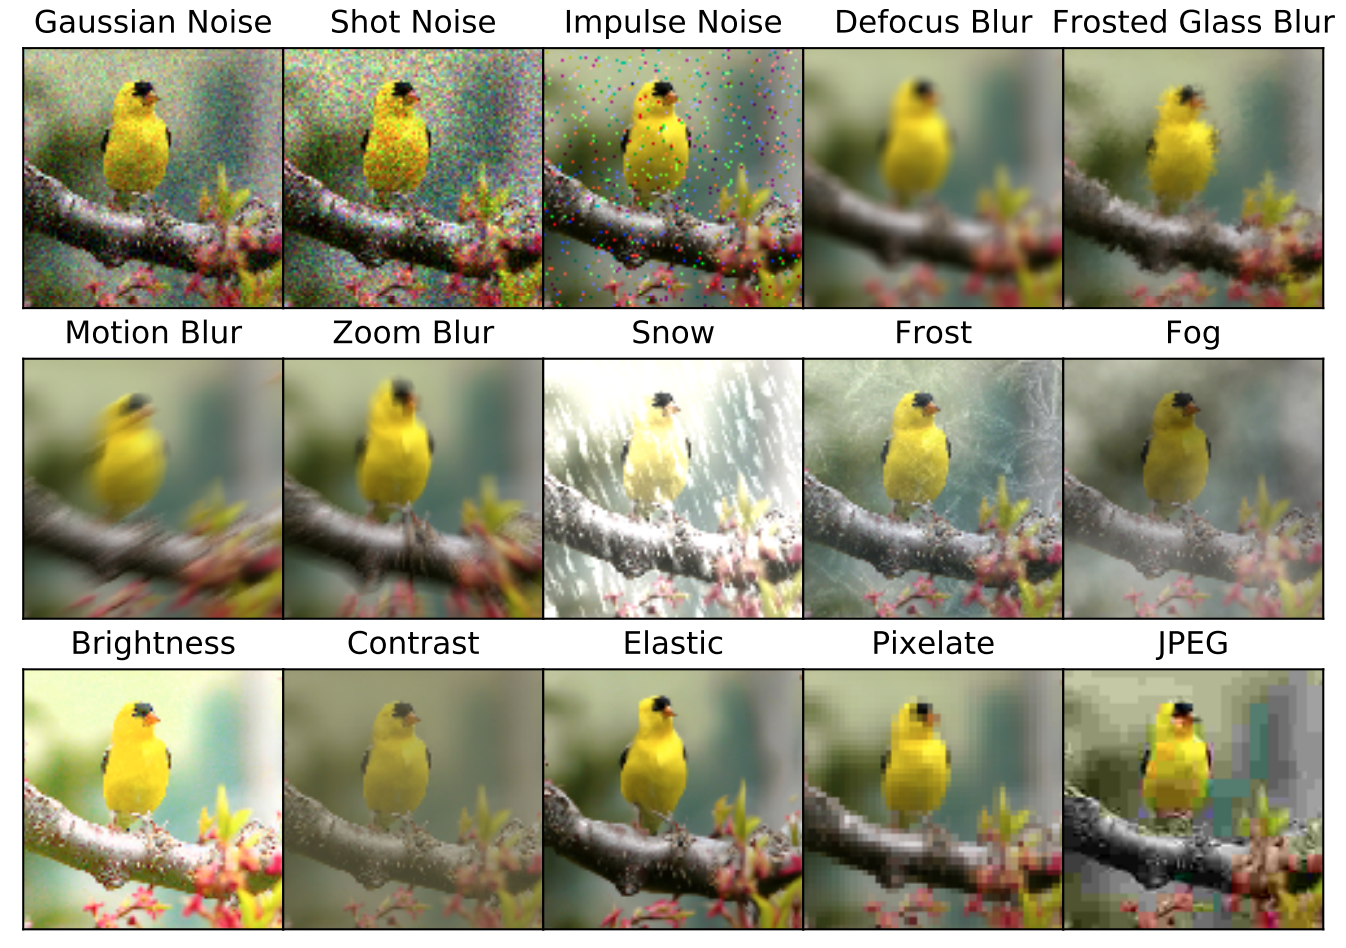
\includegraphics[width=7.5cm]{images/corruptions.png}
    \caption{Fifteen common corruptions applied to ImageNet.}
    \label{fig:corruptions}
\end{figure}

The most common metric used for ImageNet-C is \textit{mean corruption error} or mCE. To calculate mCE, divide the average error of your classifier over all corruptions by the average error of an AlexNet classifier over all corruptions. For mCE, lower is better. The authors also provide a corrupted version of the CIFAR-10 and CIFAR-100 datasets for smaller scale testing. Crucially the authors warn that \textit{networks should not be trained on ImageNet-C}. Instead, ImageNet-C is meant to act as a benchmark for a model’s robustness to an unseen dataset shift. We think that this advice can generalize to most of the benchmarks on this list.

\subsubsection{ImageNet-Sketch and ImageNet-R}
\href{https://paperswithcode.com/sota/domain-generalization-on-imagenet-sketch}{ImageNet-Sketch} \cite{wang2019learning} and \href{https://paperswithcode.com/sota/domain-generalization-on-imagenet-r}{ImageNet-R(enditions)} \cite{hendrycks2021faces} are two similar datasets also loosely based off of ImageNet. ImageNet-Sketch is a dataset which collected 50K new sketches of the various ImageNet-1k classes. ImageNet-R is a similar dataset which collected 30K renditions of various styles of the ImageNet-1k classes. Note that neither ImageNet-Sketch or ImageNet-R is a subset of ImageNet. Instead, the images are curated from new images scraped off of the internet. Examples of each dataset are shown in figure \ref{fig:renditions}.

\begin{figure}[h]
    \centering
    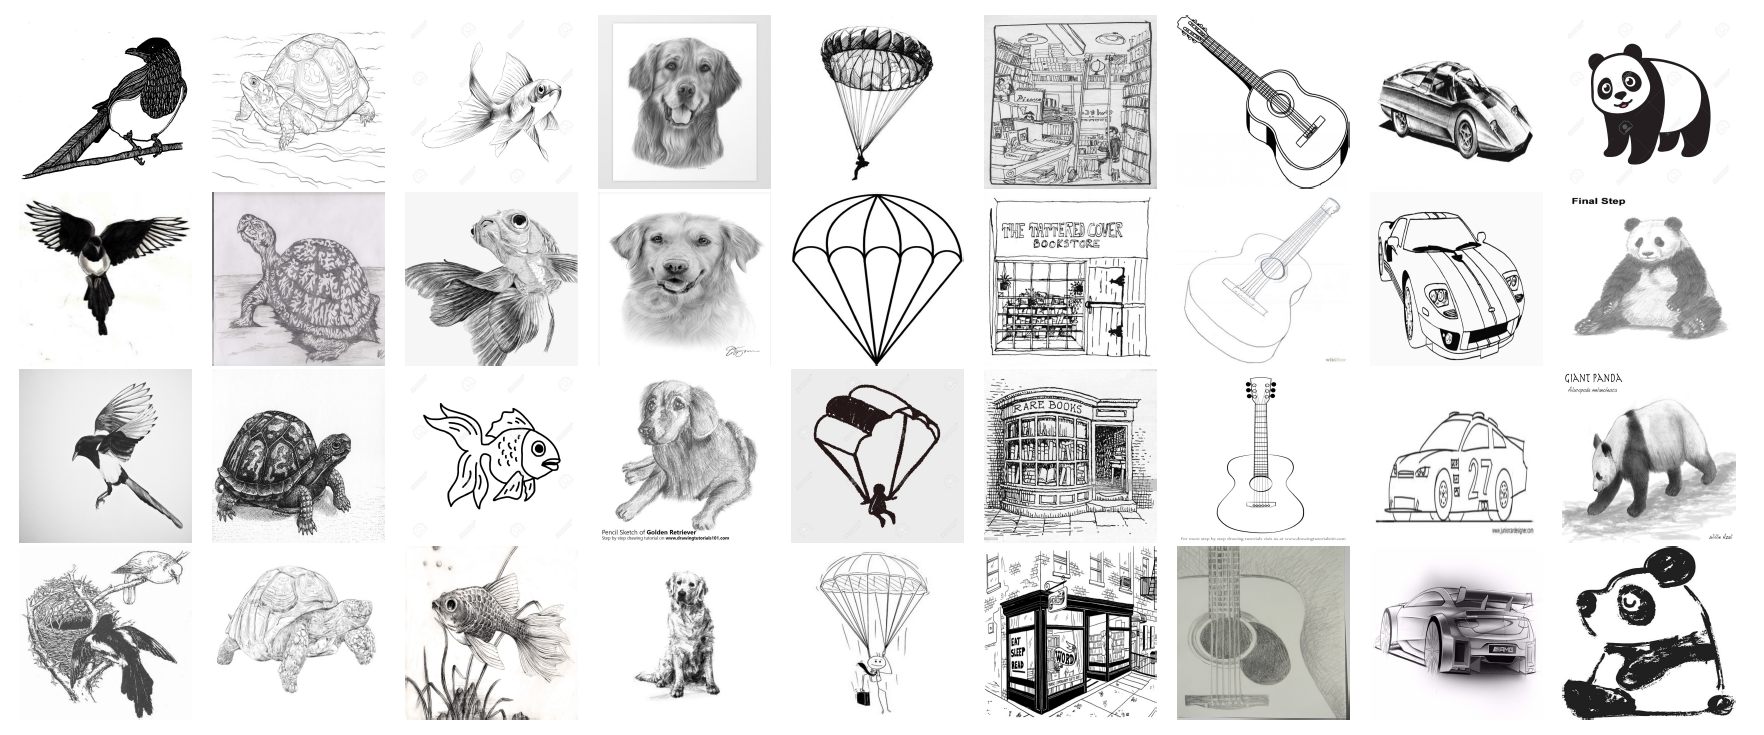
\includegraphics[width=7.5cm]{images/sketch.jpeg}
    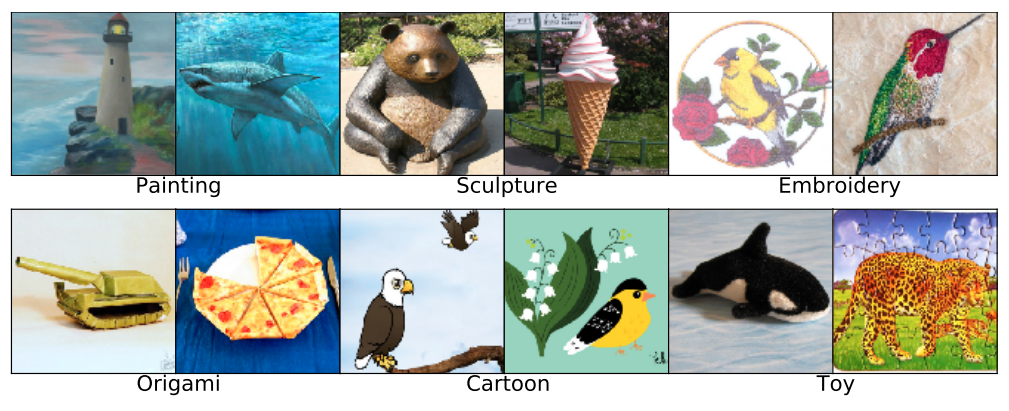
\includegraphics[width=7.5cm]{images/renditions.png}
    \caption{Example images from ImageNet-Sketch (top) and ImageNet-R (bottom).}
    \label{fig:renditions}
\end{figure}

These two datasets are designed to benchmark a model's robustness to a significant, yet still controlled, distribution shift. In particular, these datasets test whether a model can generalize from a dataset composed of largely real-world images to datasets consisting of sketches or other artistic renditions. This is a difficult task and, if achieved, provides strong evidence for a model's robustness to distribution shifts.

\subsubsection{ImageNet-A}
\href{https://paperswithcode.com/sota/domain-generalization-on-imagenet-a}{ImageNet-A} \cite{hendrycks2021natural} is a collection of images belonging to ImageNet classes, which have been adversarially filtered to be difficult for models to classify. Specifically, a large set of images are tested on two different ResNets, and only images which the ResNets both perform poorly on are included. In total, the dataset contains images spanning 200 ImageNet-1k classes. Similar to ImageNet-Sketch and ImageNet-R, ImageNet-A is also not a subset of ImageNet, but is curated from a separately collected set of images. Examples from ImageNet-A can be found in figure \ref{fig:adversarial}.

\begin{figure}[h]
    \centering
    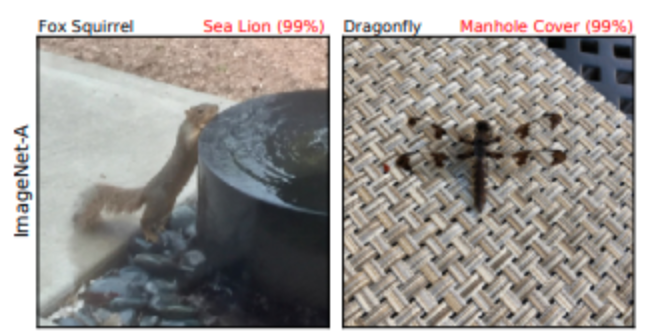
\includegraphics[width=5cm]{images/adversarial.png}
    \caption{Example images from ImageNet-A.}
    \label{fig:adversarial}
\end{figure}

\subsubsection{WILDS}
Finally, \href{https://wilds.stanford.edu/}{WILDS} \cite{koh2021wilds, sagawa2021extending} is a collection of ten datasets which document in-the-wild distribution shifts. These datasets consider distribution shift on different modalities (e.g., language, code, or molecule graphs) and in different fields (e.g., medicine, satellite pictures, Amazon reviews). In contrast with the previous benchmarks, the datasets in WILDS are unconstrained and more representative of real-world distribution shift scenarios. This means that WILDS is a good stress-test of distribution shift robustness algorithms. Furthermore, beyond the traditional $(x, y)$ pairs, WILDS provides an additional label $d$ which tells the domain of the example. The precise definition of a `domain' is task-specific, but represents a sub-distribution (e.g., all the images from a given camera) within the larger distribution. For a visualization of images in WILDS, see figure \ref{fig:wilds}.

\begin{figure}
    \centering
    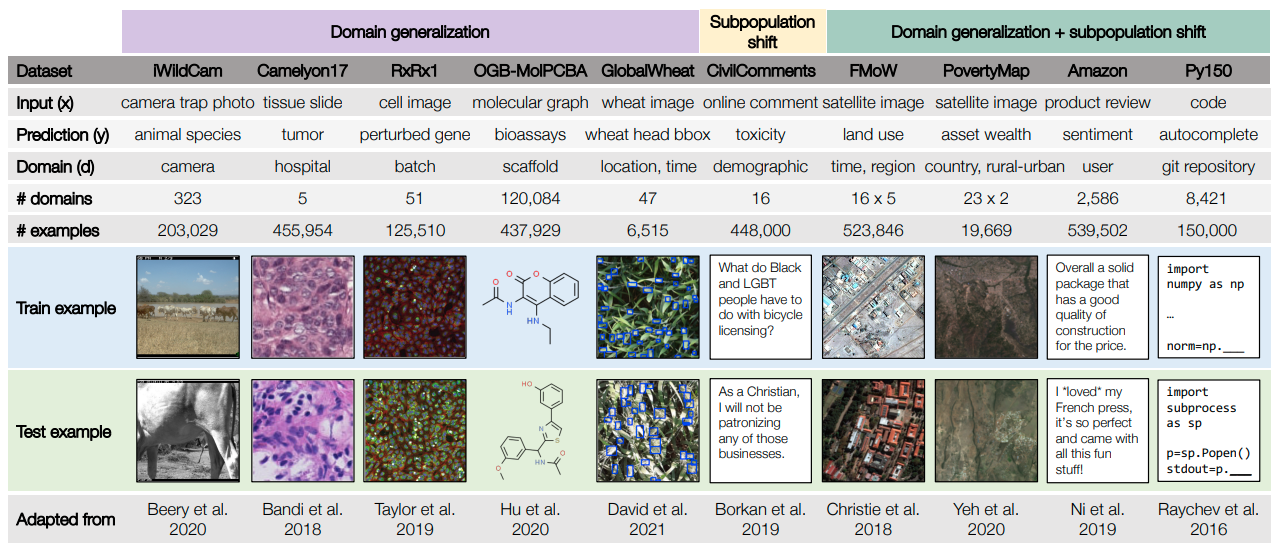
\includegraphics[width=11cm]{images/wilds.png}
    \caption{The ten different datasets in WILDS.}
    \label{fig:wilds}
\end{figure}

\section{Approaches}
Improving the robustness of ImageNet classifiers largely breaks down into three  directions: data augmentation, architectural choices, and pretraining techniques.

\subsection{Data Augmentation}
Data augmentation is the process of applying randomized transformations (e.g., horizontal flip, rotation within 30 degrees, discoloration) on input examples to create additional valid data. Data augmentation improves robustness by increasing the diversity of a dataset to include perturbed or altered images. If a model learns features robust to the data augmentation, the hope is that the same features will be robust to test-time distribution shift as well. It is important to know that in the research setting, researchers must avoid training on the exact corruptions in the testing set, else they begin to overfit on a specific set of corruptions.

Directions in data augmentation include directly proposing new augmentations \cite{zhang2018mixup, geirhos2019imagenettrained, hendrycks2021faces, hendrycks2021pixmix}, developing algorithms which find the best augmentations for any given dataset \cite{cubuk2019autoaugment, cubuk2019randaugment}, or composing multiple augmentations to further increase augmentation strength \cite{hendrycks2020augmix, hendrycks2021pixmix}. Finally, recent work has demonstrated that leveraging a specific type of adversarial data augmentation, named pyramidal adversarial training, drastically improves robustness \cite{herrmann2021pyramid}. Pyramidal adversarial training adds adversarial noise at several different resolutions, leading to an image with multiple layers of adversarial perturbation. Figure \ref{fig:pyramid} visualizes pyramid adversarial training as well as the performance gains it brings.

\begin{figure}
    \centering
    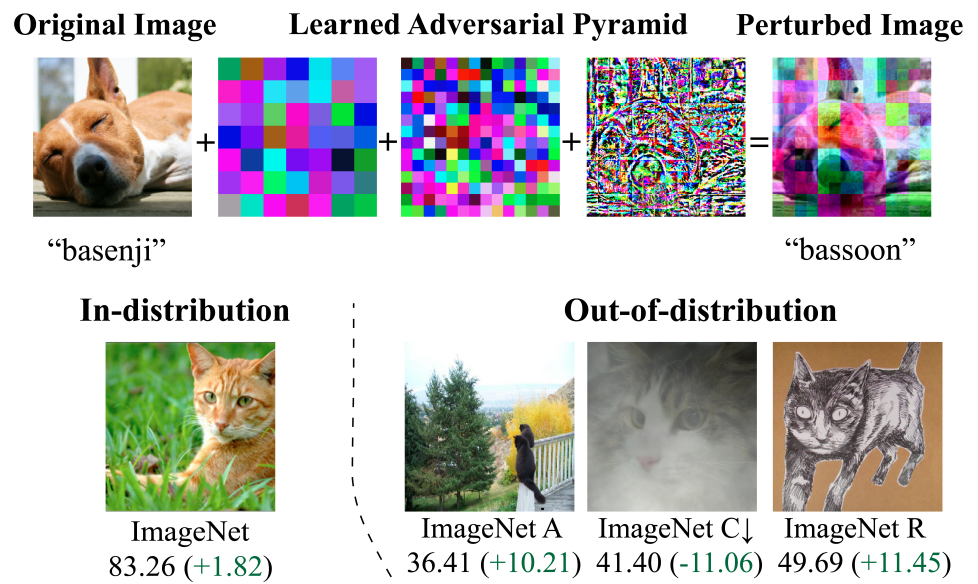
\includegraphics[width=8cm]{images/pyramid.png}
    \caption{Pyramid adversarial training improves in-distribution performance and out-of-distribution robustness.}
    \label{fig:pyramid}
\end{figure}

\subsection{Model Architecture}
Improving model architecture also leads to gains in performance. Currently, there exist two main architecture types in computer vision: convolutional neural networks and transformers. As a recap, transformers are a network architecture based heavily on ``attention,'' a technique for quickly routing information through a neural network \cite{vaswani2017attention}. Transformers were developed for natural language processing and became widespread there, before being adapted to computer vision \cite{dosovitskiy2021image}. If this is new, we highly recommend students read the initial vision transformer paper \cite{dosovitskiy2021image} or watch this \href{https://www.youtube.com/watch?v=TrdevFK_am4}{summary video}.

After the release of the initial vision transformer (ViT), researchers quickly demonstrated that vision transformers are more robust than ResNets \cite{bhojanapalli2021understanding, morrison2021exploring, paul2021vision}. ViT's robustness has been attributed to many of its architectural choices, but it's generally agreed that its attention mechanism plays a big role in its robustness. For instance, if you limit a transformer's attention to a local context, similar to the convolutional filters in a ConvNet, robustness decreases \cite{mao2021robust}. Further tweaking of the transformer led to the development of robust vision transformer (RVT). Overall, it's difficult to fully summarize RVT, as it's a collection of many small tricks which together have a very significant affect on robustness \cite{mao2021robust}. 

In the meantime, other researchers began tweaking convolutional networks as well. Researchers at Facebook released the ConvNeXt architecture \cite{liu2022convnet} which started at a ResNet50 base and systematically improved the architecture until it was on par with the best vision transformer systems. Interestingly, although they optimize for ImageNet validation performance, they get very strong robustness results as a side effect. Similar to RVT, summarizing ConvNeXt is difficult as it involves many small tricks which amount to a sizable impact. As it currently stands, RVT and ConvNeXt have similar performance on distribution shifts—neither side has established itself as the dominant architecture for model robustness just yet.

\subsection{Pretraining Techniques}
Finally, very recently, researchers have demonstrated that choosing the right pretraining technique can dramatically improve model robustness. A paper from facebook titled ``Masked Autoencoders are Scalable Vision Learners'' proposed a novel pretraining technique involving masking out large portions of the image and trying to reconstruct them. Although this core idea is nothing new \cite{vincent2008extracting, devlin2019bert}, the proposed masked autoencoder (MAE) incorporates several tricks to reach state of the art. First, MAE divides an image into patches and randomly masks out a large (around 80\%) proportion of them. In practice, aggressive masking is required, or else a model will only learn to interpolate between patches rather than learn global representations of the image. See figure \ref{fig:mae} for an example of a masked image. Second, MAE leverages vision transformers rather than convolutional networks. ConvNets are a bad choice here because each neuron has a limited receptive field, and as we previously discussed, local techniques like interpolation fail due to the aggressive masking. In contrast, vision transformers are designed to for global information aggregation and can deal with the aggressive masking better. 

Finally, MAE leverages a two-step autoencoding process for scalability. First, it uses a deep encoder to process only the non-masked patches. By only processing the patches which provide information, the encoder only needs to focus on 20\% of the image. This, in turns, enables the encoder to scale to deeper architectures. Second, it uses a shallow decoder to reconstruct the whole image. This time, the decoder inputs both the encoded vectors of the non-masked patches as well as vectors for the masked patches. However, since the decoder is much more shallow than the encoder, processing the full image ends up not being a large computational burden as well. Figure \ref{fig:mae} gives a full visualization of the architecture.

\begin{figure}
    \centering
    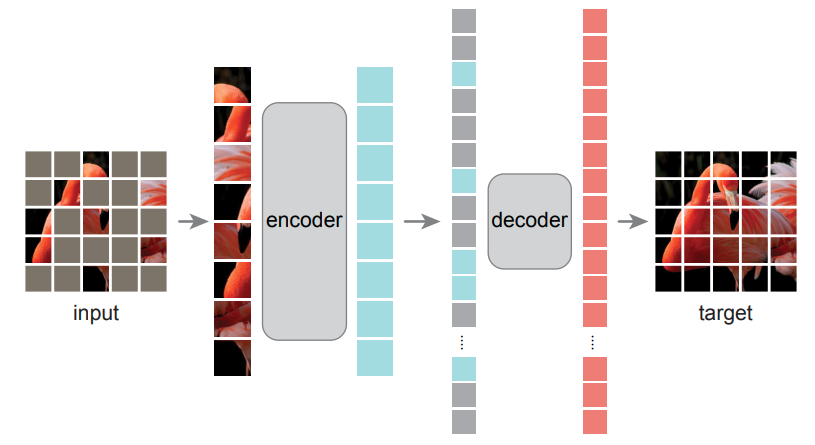
\includegraphics[width=10cm]{images/mae.png}
    \caption{MAE leverages three tricks: aggressive masking, vision transformers, and a two-part architecture for scalability. The encoder is a larger network which only processes the non-masked patches. The decoder is shallower and processes all patches, masked and non-masked. Since the encoder already has deeply processed the non-masked patches, the decoder can focus on reconstructing the image.}
    \label{fig:mae}
\end{figure}

When it was released, MAE quickly set state of the art for many robustness benchmarks, including ImageNet-C, ImageNet-Sketch, ImageNet-R, and ImageNet-A. This is attributed to two facts. First, MAE is able to scale better than other vision models, providing strong representations as model size increases. Second, MAE's pretraining technique is inherently robust, outperforming a supervised baseline by large margins when controlling for scale.

\section{Other Frameworks}
It is worth mentioning that there exists a lot of other work beyond the benchmarks and methods discussed in this set of notes. One prominent direction which has not been discussed yet involves learning features which are invariant to distribution shift \cite{arjovsky2020invariant, shi2021gradient, sun2016deep}. Specifically, this direction argues that not all correlations within the training data are valid. Instead, some correlations are spurious correlations which should be ignored by the network. For instance, a bird classification dataset may have have a correlation between being a waterbird and having a blue background \cite{sagawa2020distributionally}. However, such a correlation should be ignored by the network, as the feature `has a blue background' may not predict being a waterbird upon distribution shift. In other words, that features is not invariant to distribution shift. Work in this direction involve training auxiliary objectives to enforce feature invariance on multiple different domains \cite{arjovsky2020invariant, shi2021gradient, sun2016deep}. 

Other prominent work explores how to optimize over an explicit set of different distributions \cite{sagawa2020distributionally, subbaswamy2021evaluating}. Specifically, given knowledge of the different distributions within a dataset, this direction attempts to leverage this knowledge in the optimization algorithm. Such directions are especially relevant in the context of algorithmic bias and racial inequality \cite{buolamwini2018gender}. Finally, other work also explores robustness to label shift \cite{lipton2018detecting} or learning to adapt to a new testing distribution \cite{wang2021tent}.

\section{Conclusion}

In this chapter, we provide an exploration of one direction in distribution shift robustness. We first survey a variety of benchmarks based around ImageNet style classification. We then reviewed three areas to improve robustness: data augmentation, model architecture, and pretraining techniques. Finally, we provided a preliminary survey of other directions in distribution shift robustness.

%\todo{I think you can be a bit opinionated in the conclusion. Which directions do you think are most promising, and why? Is this an intrinsically hard problem, or is it just an issue with current architectures? How do humans solve this problem?}

\bibliographystyle{plain}
\bibliography{reference}

% Text graveyard
% 
% Distribution shift, [When the dataset shi  fts, something unseen in the testing set!]
% High level (cats breeds) vs low level (corrupted images/fog and other noise)
% This is one of the major problems in preventing wider adoptation of DL systems. (Medical stuff, self driving, social media algorithms need to deal with new vocab all the time.)
% We focus on image classification, specifically large scale, everyday object classification based around ImageNet. [Discussion on benchmarks?]
% Also, there are a lot of different frames to take this. Domain Adaptation, Test time adaptation, etc, etc.
%For instance, imagine you’re a medical practitioner looking to train an image classifier on MRI scans. Collecting and labeling MRI scans is quite expensive (requires hiring medical professionals), so instead you’re likely to leverage publicly labeled MRI datasets. However these publicly available datasets are a different distribution than your own—maybe your hospital has different demographics than are represented in the public dataset, maybe your MRI scanning equipment is slightly different and therefore produces slightly different images. In order for an image classifier to be useful, you need to achieve high performance despite the shift in distribution.
%[Image—public dataset vs your dataset (demographics, scanning equipment, performance degrades). Have an example image in each, with the factors at the bottom/top and a performance degrades]

%In the last chapter we looked at detecting out-of-distribution data to understand when a model’s predictions may be faulty or incorrect. However, in many situations, simply detecting out-of-distribution data isn’t enough—instead, we want to have high performance on this out-of-distribution data. 

% https://arxiv.org/pdf/2106.10270.pdf
%\subsection{Increasing Dataset Size}
%It turns out that simply increasing dataset size improves model robustness on a variety of benchmarks \cite{steiner2021train}. For instance, training on ImageNet-1k (1.3 million images) is less effective than training on ImageNet-21k (14 million images) which in turn is less effective than training on Google’s JFT-300M (300 million images). 

%[Create Image]

%The increased dataset size improves the diversity of images seen in the dataset, resulting in features which are more robust to novel images. This knowledge, however, is not useful for researchers who do not have the resources to build an even larger image dataset or for practitioners who do not have access to JFT-300M (as it is private). Instead, given a limited dataset, a more practical way of improving model robustness is to leverage data augmentation.

%Data augmentation can be viewed as a way to artificially expand the dataset. Similar to increasing dataset size, this increases the diversity of images in the dataset resulting in more robust features. AugMix is an example technique which improves robustness by using data augmentations to diversify the dataset. AugMix takes an image $x$ and generates some number of augmented images $x_1, ..., x_k$ where each xi is created by sampling and chaining together some number of augmentations. AugMix then recombines the augmented images $x_1, ..., x_k$ by taking a weighted average. Finally, the resultant image is also recombined with the original image in another weighted average. This is shown visually in figure \ref{fig:augmix}.

%\begin{figure}
%    \centering
%    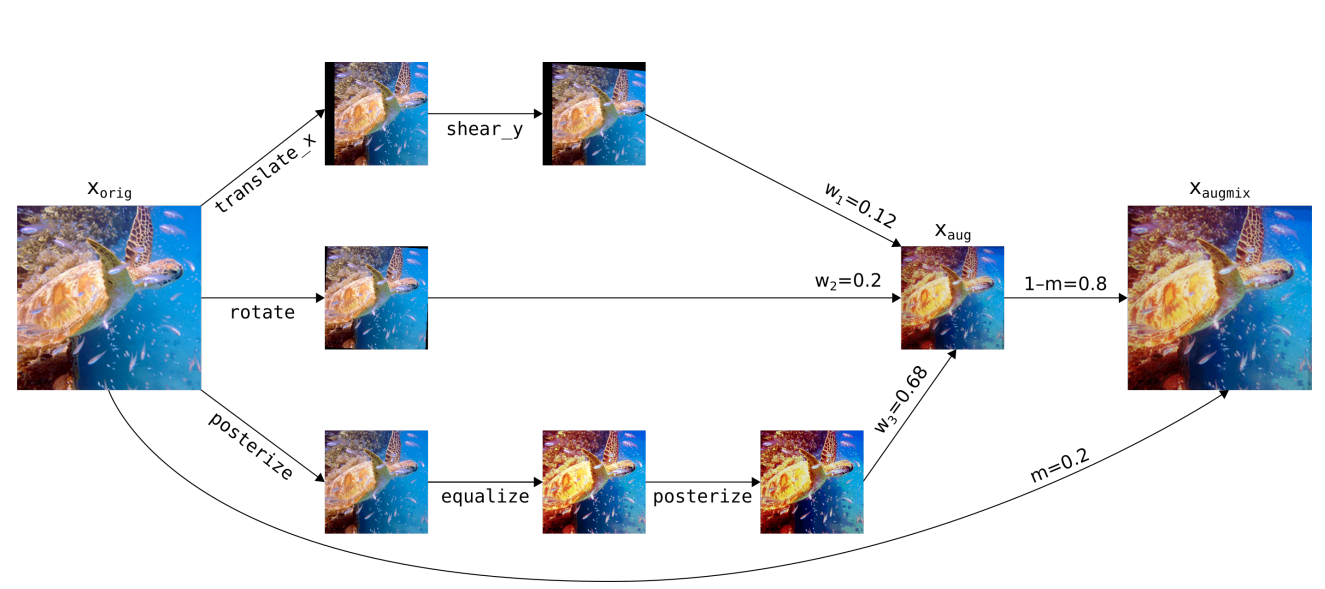
\includegraphics[width=7.5cm]{images/augmix.png}
%    \caption{AugMix augments the turtle using $k=3$ chains. Then the augmented images are combined using a weighted average. Finally, the combined image and the original image are also combined.}
%    \label{fig:augmix}
%\end{figure}

%By chaining together lots of individual augmentations, AugMix is able to consistently create novel and unexpected images for the model. This helps the model build robust features for downstream tasks. Empirically, AugMix decreased mCE on ImageNet-C by 10 percentage points compared to a baseline.

%For instance, MixUp is an augmentation which creates new augmented samples by interpolating between pre-existing samples \cite{zhang2018mixup}. Given datapoints $(x_1, y_1)$ and $(x_2, y_2)$, we sample $\lambda \in [0, 1]$ to generate new datapoint $\lambda x_1 + (1-\lambda) x_2$ with label $\lambda y_1 + (1-\lambda) y_2$. See figure  

% Data Augmentation
% Pyramidal adversarial training
\end{document}
